\newpage
\section{Aufbau}
\label{sec:aufbau}

\begin{figure}
    \centering
    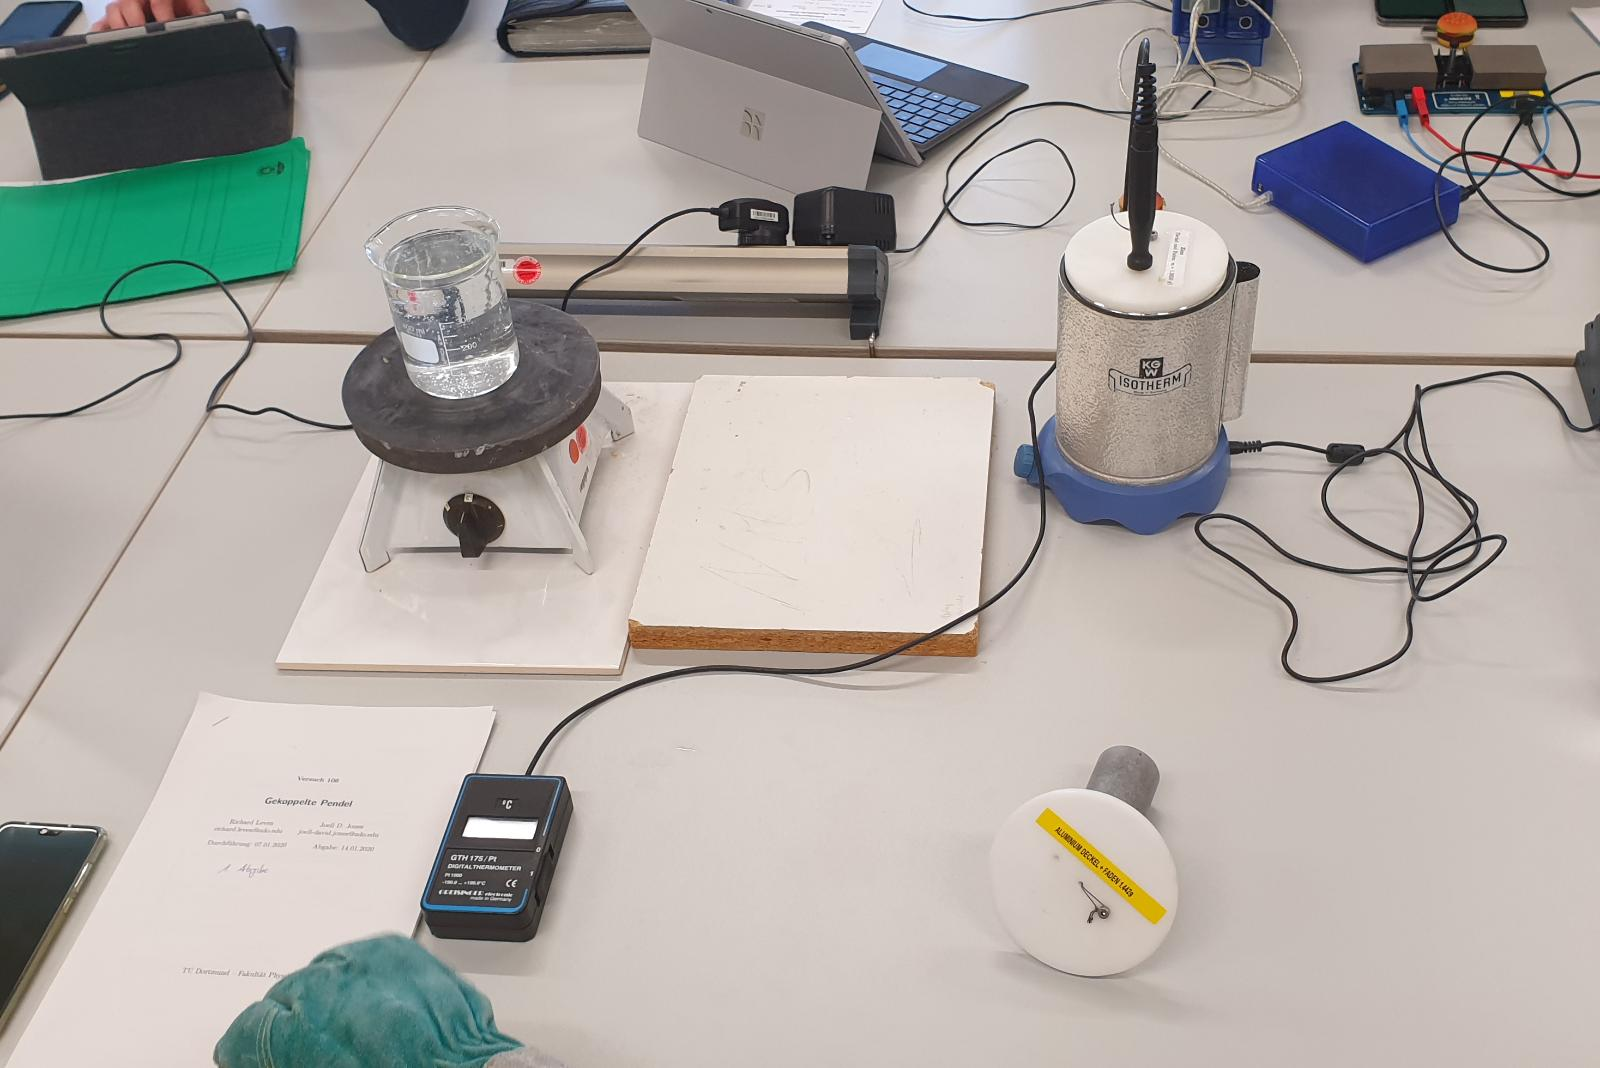
\includegraphics[scale=0.1]{content/Bilder/Aufbau.jpg}
    \caption{Aufbau der Schaltung und des Versuchsapperats.}
    \label{fig:aufbau}
\end{figure}
Der Aufbau des Experiments zur Bestimmung des Torsionsmoduls G ist in \autoref{fig:aufbau2} dargestellt.
\begin{figure}
    \centering
    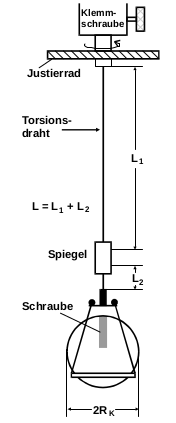
\includegraphics[width=0.3\textwidth]{content/Bilder/Torsion.png}
    \caption{Aufbau der Drehschwingung \cite{v102}.}
    \label{fig:aufbau2}
\end{figure}
Eine erweiterte Form davon beinhaltet ein Helmholtz-Spulenpaar, wie in \autoref{fig:aufbau3} zu sehen ist:
\begin{figure}
    \centering
    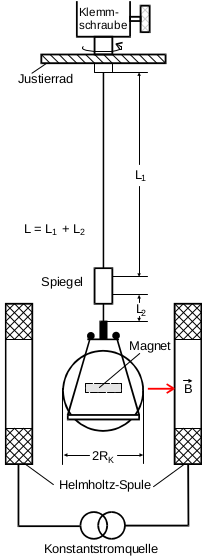
\includegraphics[width=0.3\textwidth]{content/Bilder/Magnet.png}
    \caption{Aufbau der Drehschwingung mit Helmholtz-Spulen \cite{v102}.}
    \label{fig:aufbau3}
\end{figure}